\documentclass[a4paper,11pt]{article}
%@@@@@@@@@@@@@@@@@@@@@@@@@@@@@@@@@@@@@@@@@@@@@@@@@@@@@@@@@@@
%@@@@@@@@@@@@@@@@      PACOTES BÁSICOS		     @@@@@@@@@@
%@@@@@@@@@@@@@@@@@@@@@@@@@@@@@@@@@@@@@@@@@@@@@@@@@@@@@@@@@@@

\usepackage[T1]{fontenc}
\usepackage[utf8]{inputenc}
\usepackage{lmodern} 
\usepackage[portuguese]{babel}
\usepackage{amsmath}
\usepackage{array}
\usepackage{graphicx}				%para imagens
\usepackage{epstopdf} 				%resolve problemas eps-pdf
\usepackage{pict2e}				%%writting to images
%@@@@@@@@@@@@@@@@@@@@@@@@@@@@@@@@@@@@@@@@@@@@@@@@@@@@@@@@@@@
%@@@@@@@@@@@@@@@@     PACOTES NÃO TAOBÁSICOS		 @@@@@@@@@@
%@@@@@@@@@@@@@@@@@@@@@@@@@@@@@@@@@@@@@@@@@@@@@@@@@@@@@@@@@@@
\usepackage{fancyhdr}				% para o cabeçalho bonito
\usepackage{caption}					%para legendas
\usepackage{subcaption}				% e sublegendas
\usepackage{placeins} 				%controlar o lugar dos floats
\pagestyle{fancy} 					% número de pag e cabeçalho
\usepackage{txfonts} 				%fontes bonitas? acho que para o título
\usepackage[usenames]{color} 		% algo com gunplot e eps
\usepackage{ifthen}
\usepackage{xparse}
\graphicspath{{./../images/}{./../data/}{./graph/}}	% procura imagens nessa pasta
\usepackage{float} %%para definir ambiente gráfico
\newfloat{Gráfico}{hbtp}{lop}[section]
%\usepackage{undertilde}	%%para notação de vetor do yuri
\usepackage[import]{xy} % para escrever em imagens
\xyoption{import}

\usepackage{listings}
\lstset{frame=single,}
%@@@@@@@@@@@@@@@@@@@@@@@@@@@@@@@@@@@@@@@@@@@@@@@@@@@@@@@@@@@
%@@@@@@@@@@@@@@@@      Cabeçalho de cada página      @@@@@@@
%@@@@@@@@@@@@@@@@@@@@@@@@@@@@@@@@@@@@@@@@@@@@@@@@@@@@@@@@@@@
\setlength{\headheight}{25pt}%compila sem erro
	\fancyhead{}
	\fancyfoot{}
	\fancyhead[R]{Sistemas de Medição}%direito superior
	\fancyhead[L]{
\includegraphics[height=0.25in]{./../images/logo_unb.pdf}}%esquerda superior
	\fancyfoot[C]{\thepage}%baixo centro
%E: Even page, O: Odd page, L: Left field, C: Center field, R: Right field, H: Header, F: Footer
% em documentos com dois lados use LO, RO. como esse documento não tem lados essa opção é inútil


%@@@@@@@@@@@@@@@@@@@@@@@@@@@@@@@@@@@@@@@@@@@@@@@@@@@@@@@@@@@
%@@@@@@@@@@@@@@@@      NOVOS COMANDOS		      @@@@@@@@@
%@@@@@@@@@@@@@@@@@@@@@@@@@@@@@@@@@@@@@@@@@@@@@@@@@@@@@@@@@@@
\newcommand\undermat[2]
	{
	  \makebox[0pt][l]
	  	{$\smash{\underbrace{\phantom{%
    \begin{matrix}#2\end{matrix}}}_{\text{$#1$}}}$
    		}#2
    	}
    	
\newcommand{\HRule}
	{
	\rule{\linewidth}{0.5mm}
	}
	
\newcommand{\EmptyPage}
	{
	\thispagestyle{empty}
	\mbox{ }
	\newpage	
	} 
	
\newcommand{\MakeMyTitlePage}[4]
%%Argumentos: 
%1º Nome da Matéria
%2º subtítulo ex: experimento IV
%3º título
%4º autores
% exemplo de autores:
%	\begin{center} \large
%		\begin{tabular}{llr} \
%		& & \\[0.05cm]		
%		Professora & Nadia Maria de Liz Koche & \\
%		
%		Alunos:& & \\
%		& Juarez A.S.F 					& 11/0032829\\
%		& Sérgio Fernandes da Silva Reis & 11/0140257\\
%		& Jedhai Pimentel				& 09/0007883\\	[0.05cm]	
%		\end{tabular}
%	\end{center}
{
\begin{titlepage}
\begin{center}

% Upper part of the page. The '~' is needed because \\
% only works if a paragraph has started.

\includegraphics[width=\textwidth]{./../images/logo_unb.pdf}~\\[1cm]

\Huge #1\\[0.5cm]

\huge #2

% Title
\HRule \\[0.4cm]
{ \huge \bfseries  #3}\\[0.4cm]

\HRule \\[0.5cm]

{\large \today}


\vfill %%o que vier depois vai ao fim da páginda


%Autor e Professor
\begin{center} \large
#4
\end{center}

\end{center}
\end{titlepage}

\EmptyPage
\tableofcontents
\newpage

}
	
%@@@@@@@@@@@@@@@@@@@@@@@@@@@@@@@@@@@@@@@@@@@@@@@@@@@@@@@@@@@
%@@@@@@@@@@@@@@@@      NOVOS AMBIENTES		      @@@@@@@@@
%@@@@@@@@@@@@@@@@@@@@@@@@@@@@@@@@@@@@@@@@@@@@@@@@@@@@@@@@@@@
\newcounter{graph-c}
\setcounter{graph-c}{0}


%\NewDocumentEnvironment{Graph}{m}
 % {%antes
  %\addtocounter{graph-c}{1}
  %\begin{figure}
  %}
 %{
 %depois
%	\end{figure} 
%	\caption*{Grafico \arabic{graph-c} - #1}
 %}

















%inclui todosos pacotes utilizados

\begin{document}



\MakeMyTitlePage
{Física Experimental 4}
{Experimento VI-a}
{O caráter quântico da luz e a constante de Planck}
{%autores
		\begin{tabular}{llr} \
		& & \\[0.05cm]		
		Professora & Nadia Maria de Liz Koche & \\
		
		Alunos:& & \\
		& Juarez A.S.F 					& 11/0032829\\
		& Jedhai Pimentel				& 09/0007883\\
	[0.05cm]	
		\end{tabular}
}

%@@@@@@@@@@@@@@@@@@@@@@@@@@@@@@@@@@@@@@@@@@@@@@@@@@@@@@@@@@@
%@@@@@@@@@@@@@@@@      OBJETIVOS      @@@@@@@@@@@@@@@@@@@@@@
%@@@@@@@@@@@@@@@@@@@@@@@@@@@@@@@@@@@@@@@@@@@@@@@@@@@@@@@@@@@
\section{Objetivos}
\paragraph{}Verificar a validade das hipóteses quânticas e
clássica da luz estudando o efeito fotoelétrico. Determinar 
a constante de Planck e a função trabalho do fotodiodo.
%@@@@@@@@@@@@@@@@@@@@@@@@@@@@@@@@@@@@@@@@@@@@@@@@@@@@@@@@@@@
%@@@@@@@@@@@@@@@        MATERIAIS         @@@@@@@@@@@@@@@@@@
%@@@@@@@@@@@@@@@@@@@@@@@@@@@@@@@@@@@@@@@@@@@@@@@@@@@@@@@@@@@
\section{Materiais}
\paragraph{} Para o experimento utiliza-se:
\begin{itemize}
  \item Voltímetro digital
  \item Módulo h/e(AP-9368) da Pasco
  \item Kit de acessórios para o módulo h/e (AP-9368) da
    Pasco
  \item Fonte de luz de vapor de mercúrio (OS-9286) da Pasco
  \item filtros de verde e de amarelo
  \item filtro de transmissão variável com percentagens de
    100\%, 60\%, 40\% e 20\%
  \end{itemize}

%@@@@@@@@@@@@@@@@@@@@@@@@@@@@@@@@@@@@@@@@@@@@@@@@@@@@@@@@@@@
%@@@@@@@@@@@@@@        INTRODUCAO       @@@@@@@@@@@@@@@@@@@@
%@@@@@@@@@@@@@@@@@@@@@@@@@@@@@@@@@@@@@@@@@@@@@@@@@@@@@@@@@@@
\newpage
\section{Introdução}

\paragraph{}O entendimento físico da luz como uma onda
eletromagnética explica vários fenômenos como a refração,
reflexão, difração e interferência. No entanto, um modelo puramente ondulatório
falha em descrever corretamente algumas outras propriedades
e efeitos da luz. Uma dessas falhas do modelo ondulatório é
explicar o efeito fotoelétrico.

\paragraph{}O efeito fotoelétrico ocorre quando sólidos,
líquidos ou gases emitem elétrons ao absorverem energia da
luz.
Tais elétrons são chamados de fotoelétrons. O modelo
ondulatório prevê que a energia cinética desses elétrons, e
portanto sua velocidade, dependem exclusivamente da
intensidade da luz incidente. Ou seja, dadas duas ondas
incidentes em um material o modelo clássico diz que a onda que possuir maior
amplitude irá liberar elétrons com maior energia. Tal
previsão, no entanto, não se verifica experimentalmente.
Para explicar corretamente o efeito é preciso adotar o
modelo quântico para a luz.

\paragraph{}O modelo quântico diz que a emissão de luz
ocorre de forma discreta em pacotes de energia, os fótons, e que a
energia E que cada
pacote desse possui está relacionada com a frequência
$\nu$ da onda
pela fórmula:
\begin{equation}
E = h\nu
\end{equation}
onde h é uma constante universal conhecida como constante de
Planck. Por exemplo, em uma luz monocromática todos os
fótons terão a mesma energia individual e uma luz mais
intensa carregará apenas uma quantidade maior de fótons. É
justamente esse entendimento que irá explicar o efeito
fotoelétrico. A liberação de elétrons pelos átomos de um
material nesse efeito ocorre devido a interação individual de um
elétron com um fóton. Quando a energia absorvida pelo
elétron for maior do que aquela que o prende ao
átomo, o elétron será liberado e o restante da
energia, se houver, será convertido em energia cinética.
Veja que se existirem mais fótons colidindo com o material
teremos mais das mesmas interações de um fóton com um elétron,
de modo que teremos mais elétrons liberados e todos com a
mesma energia. Dessa forma, a  energia dos elétrons liberados
depende da energia dos fótons incidentes e portanto da
frequência da luz incidente e não da sua intensidade.

\paragraph{}Seja $h\nu$ a energia do fóton incidente e
$W_0$ a energia necessária para arrancar o elétron do átomo,
conhecida como função trabalho. A energia cinética com que o
fotoelétron de massa m deixa o átomo após absorver o fóton é:
\begin{equation}
  \frac{1}{2} mv^2 = h\nu - W_0
  \label{eq:einstein}
\end{equation}

\paragraph{} Vamos usar essa equação para determinar a
constante de Planck.
Considere a figura \ref{fig:efeitoFE}. Se os
fótons incidentes tiverem energia o suficiente para que os
elétrons arrancados da superfície do catodo consigam chegar
ao anodo temos uma corrente fotoelétrica no interior do
tubo. Se o circuito se mantiver aberto a medida que isso
ocorre começaremos a ter um acúmulo de carga no anodo,
gerando uma ddp que tende a frear os elétrons da corrente
fotoelétrica. Quando esse potencial acumulado for alto o
suficiente para que a energia potencial $eV$ iguale a energia
cinética $\frac{1}{2}mv^2$ com que os
elétrons deixam o catodo teremos equilíbrio e a corrente
fotoelétrica cessa. Medindo o potencial $V_{max}$ em que a corrente
cessa e usando a fórmula \ref{eq:einstein} podemos obter:
\begin{equation}
  V_{max} = \frac{h}{e}\nu - \frac{W_0}{e}
  \label{eq:IMPORTANTE}
\end{equation}

\paragraph{}Vemos que de um gráfico da tensão de parada da
corrente pela frequência incidente pode-se obter a constante 
de Planck, uma vez que se conheça a carga do elétron. Nessa
análise consideramos que o circuito é deixado em aberto para
que toda carga que chegue ao anodo seja acumulada, no
entanto, se
colocarmos um voltímetro real nas extremidades para medir o
dado necessário para a construção do gráfico estaremos
fechando um circuito e as cargas negativas do anodo podem
retornar ao catodo. Como a resistência do voltímetro deve
ser muito grande, essa volta de cargas ocorre de maneira
lenta, de modo que ainda assim é possível observar o fim da
corrente fotoelétrica. Esse fato, no entanto, deve ser levado
em consideração para melhor entender os dados experimentais.
\FloatBarrier
\begin{figure}[!htp]
    \centering
    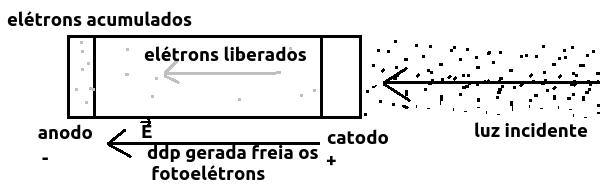
\includegraphics[scale = 0.5]{./images/foto-eletric.jpeg}
    \caption{Modelo para efeito fotoelétrico: lembre que os
    elétrons são empurrados na direção contrária ao campo
    $\vec{E}$}
    \label{fig:efeitoFE}
\end{figure}
\FloatBarrier
\newpage
\section{Procedimentos}
\paragraph{} O procedimento é dividido em duas etapas: na
primeira verificamos o comportamento da tensão máxima em
função da intensidade incidente e na segunda em função da
frequência incidente.

\paragraph{}Inicialmente deve-se ajustar a montagem para que
a fenda e o fotodiodo estejam alinhados. Considere a
montagem na figura \ref{fig:proced}.Liga-se a lâmpada de
mercúrio e remove-se o cano
do fotodiodo. Posiciona-se o braço móvel para que uma
das raias espectrais atinja a fenda de entrada. Nessa posição
deve-se posicionar o fotodiodo girando-o em torno de seu eixo de forma que
a luz que passa da fenda cubra toda a área sensível do
fotodiodo. Feito isso fecha-se o cano e mantem-se essa
configuração do fotodiodo para o resto do experimento.

\paragraph{Relação com a intensidade} Agora posiciona-se 
o braço móvel de forma que a primeira raia
espectral(violeta forte) atinja a fenda de entrada do fotodiodo.
Prende-se então o filtro de intensidade na fenda de entrada.
Primeiramente posiciona-se o filtro para que sua porção de
transmissão de 100\% esteja sobre a fenda. Zera-se o
potencial do fotodiodo com o botão em sua lateral e,
depois de soltado o botão, espera-se para que o potencial
se estabilize. O potencial estabilizado é anotado e o
procedimento é refeito para todas as percentagens do filtro.
Repete-se o procedimento para todas as faixas de primeira
ordem do espectro(até o primeiro amarelo). Na medição
da faixa verde deve-se acoplar ainda o filtro verde, e na
amarela um filtro amarelo. Isso é feito para evitar
interferências de frequências próximas. O acoplamento desses
filtros pode ser feito colocando-se um suporte para filtros
no caminho do feixe correspondente.

\paragraph{Relação com a intensidade} Retira-se agora o
filtro de intensidade da fenda. Posiciona-se o braço fixo 
na primeira raia espectral(violeta forte)
\footnote{De fato
essa primeira raia corresponde ao ultravioleta emitido pela
fonte de mercúrio. Essa frequência, no entanto, sofre
alteração pela rede de difração e aparece aqui como visível}
e, depois de zerado o potencial, mede-se o potencial máximo 
mostrado pelo multímetro. O procedimento é refeito para
todas as raias de primeira ordem. Novamente usam-se os
filtros de verde a amarelo nas medidas relativas a essas
cores.

\FloatBarrier
\begin{figure}
  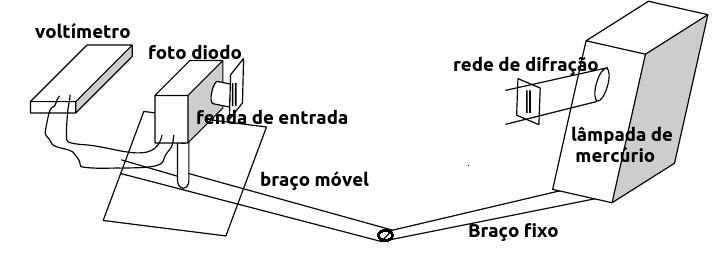
\includegraphics[scale=0.5]{./images/montagem.jpeg}
  \caption{Montagem do procedimento}
  \label{fig:proced}
\end{figure}
\FloatBarrier

\section{Dados}
\paragraph{}Os dados do primeiro procedimento são 
mostrados na tabela \ref{tab:A} e do segundo na tabela
\ref{tab:B}. Na tabela dois os comprimentos de onda 
aparecem na mesma ordem em que as cores da tabela
\ref{tab:A} e foram obtidos do fabricante da lâmpada de
mercúrio.

\paragraph{}Além desses dados quantitativos acrescentamos
que na primeira etapa quanto menor era a intensidade
do filtro mais demorava para o voltímetro estabilizar.
\begin{table}[!htp]
    \centering
    \hspace{-10 cm}
    \parbox{.45\linewidth}
		{
		\begin{tabular}{|l|l|l|l|l|l|}\hline
          intensidade(\%) & $V_{max}$(V)ultravioleta &
          $V_{max}$(V) violeta &
         $V_{max}$    azul &  $V_{max}(V)$verde &
         $V_{max}$(V)amarelo\\ \hline
					 1497 &  1.0060 \\ \hline 
		 1037 &  1.0140 \\ \hline 
		 869 &  1.0155 \\ \hline 
		 703 &  1.0185 \\ \hline 
		 548 &  1.0220 \\ \hline 
		 401 &  1.0240 \\ \hline 
		 249 &  1.0255 \\ \hline 
		 111 &  1.0275 \\ \hline 
		 -111 &  1.0320 \\ \hline 
		 -258 &  1.0350 \\ \hline 
		 -402 &  1.0378 \\ \hline 
		 -555 &  1.0405 \\ \hline 
		 -699 &  1.0428 \\ \hline 
		 -856 &  1.0448 \\ \hline 
		 -1004 &  1.0485 \\ \hline 
		 -1517 &  1.0575 \\ \hline 

		\end{tabular}
        \caption{$V_{max}$ em função da intensidade}
		\label{tab:A}
		}

\parbox{.45\linewidth}
		{
		\centering
		\begin{tabular}{|l|l|}\hline
          frequência($10^{14}$Hz) & $V_{max}(V)\pm 0.001$ \\ \hline
					 5.18672 &  0.830 \\ \hline 
		 5.48996 &  0.951 \\ \hline 
		 6.87858 &  1.587 \\ \hline 
		 7.40858 &  1.761 \\ \hline 
		 8.20264 &  1.996 \\ \hline 

		\end{tabular}
        \caption{$V_{max}$ em função da frequência}
		\label{tab:B}
		}

\end{table}

\newpage
\section{Análise de Dados}
\paragraph{} Os dados da primeira etapa são plotados no
gráfico \ref{graph:A}. Os pontos experimentais
estão marcados em círculos e a reta pontilhada une os pontos
para mostrar o comportamento quase constante de
$v_{max}$, o que já era possível ver da própria tabela
\ref{tab:A}. Vemos aqui que o comportamento não é o ideal
previsto pelo modelo quântico pois quando a intensidade é
muito baixa observamos uma queda no potencial de parada para
todas as cores observadas. Isso se deve ao fato notado
na introdução de que ao ligarmos o voltímetro em paralelo
para medir o potencial fechamos o circuito e parte das
cargas negativas acumuladas podem voltar para o catodo. Para
explicar como isso afeta as medidas vamos fazer uma analogia 
com uma torneira que enche uma banheira vazada. Em nosso
caso a mangueira é a corrente fotoelétrica, a água da
banheira é o potencial acumulado e o ralo é o circuito
fechado pelo multímetro. Em nossa analogia a banheira estará
cheia quando o potencial acumulado for o potencial de
parada. Em todos os casos estudados o ralo é o mesmo mas
muda a vazão com que a mangueira injeta água na banheira. Ou
seja, desde que a vazão de entrada seja maior que a vazão de
saída temos certeza de que uma hora a banheira estará cheia,
mas quanto menor for a vazão de entrada mais tempo isso
demorará para acontecer. É o que ocorre aqui, quanto maior a
intensidade da corrente fotoelétrica mais rapidamente o
potencial de parada é atingido. Se em nossas medidas
tivéssemos esperado tempo suficiente,  teríamos todos os
$V_{max}$ iguais, independentemente da intensidade
incidente.

\paragraph{}Para concluir, notamos que esse procedimento
mostra que o potencial de parada, e portanto a energia
cinética dos fotoelétrons, não depende da intensidade
incidente, uma vez que esta se manteve constante para
todas as percentagens de transmissão utilizadas. Esse
procedimento discorda portanto das previsões da física
clássica.



\paragraph{}Os dados da segunda etapa são plotados no gráfico
\ref{graph:B}. A regressão para os dados do segundo gráfico 
é:

\begin{equation}
  V_{máx} = (0.0000000000000037 \pm 0.0000000000000003) \nu - (1.0 \pm 0.2)

  \label{eq:FitB}
\end{equation}

comparando com a fórmula \ref{eq:IMPORTANTE} da introdução
obtemos:
\begin{displaymath}
  \begin{array}{l}
    \frac{h}{e} = (3.7 \pm 0.3)\cdot 10^{-15}V\cdot s \\
    \frac{W_0}{e} = (1\pm0.2)V
    \end{array}
\end{displaymath}

conhecendo a carga do elétron $e = 1.602 \cdot
10^{-19}$C podemos então determinar a constante de tempo
a partir do coeficiente angular.
\begin{equation}
  \MyBox{$h = (5.9\pm 0.5) \cdot 10^{-34}V \cdot C \cdot s $}
\end{equation}

onde a propagação do erro foi feita utilizando-se:

\begin{equation}
  \triangle h = e\triangle \frac{h}{e}
\end{equation}

analogamente, obtemos a função trabalho a partir do
coeficiente linear:
\begin{equation}
  \MyBox{$W_0 = (1.6\pm 0.3) \cdot 10^{-19}V \cdot C$}
\end{equation}

onde a propagação do erro foi feita utilizando-se:

\begin{equation}
  \triangle W_0 = e\triangle \frac{W_0}{e}
\end{equation}

\paragraph{}Aqui apresentamos os resultados em unidades SI,
mas se quiséssemos apresentar em eV bastaria pegar os
próprios coeficientes da reta, uma vez que a equação já está
dividia por e.

\paragraph{}Os erros percentuais são: 6.76\% para a
constante de Planck e 18.74\% para a função trabalho.
O valor tabelado para a constante de Planck é de $6.62606896
\cdot 10^{-34}$, que não cai dentro da margem de erro
calculada. Portanto a medida da constante de Planck foi
precisa mas não acurada. Quanto a medida da função trabalho
esta apresentou uma grande margem de erro, portanto foi não
precisa.

\paragraph{}Notamos que esse procedimento apoia a teoria
quântica ao verificar que o potencial de parada está
relacionado de forma linear com a frequência incidente.

\FloatBarrier

\begin{figure}
  \begin{subfigure}{\linewidth}
         % GNUPLOT: LaTeX picture with Postscript
\begingroup
  \fontfamily{phv}%
  \selectfont
\definecolor{t}{rgb}{0.5,0.5,0.5}
  \makeatletter
  \providecommand\color[2][]{%
    \GenericError{(gnuplot) \space\space\space\@spaces}{%
      Package color not loaded in conjunction with
      terminal option `colourtext'%
    }{See the gnuplot documentation for explanation.%
    }{Either use 'blacktext' in gnuplot or load the package
      color.sty in LaTeX.}%
    \renewcommand\color[2][]{}%
  }%
  \providecommand\includegraphics[2][]{%
    \GenericError{(gnuplot) \space\space\space\@spaces}{%
      Package graphicx or graphics not loaded%
    }{See the gnuplot documentation for explanation.%
    }{The gnuplot epslatex terminal needs graphicx.sty or graphics.sty.}%
    \renewcommand\includegraphics[2][]{}%
  }%
  \providecommand\rotatebox[2]{#2}%
  \@ifundefined{ifGPcolor}{%
    \newif\ifGPcolor
    \GPcolortrue
  }{}%
  \@ifundefined{ifGPblacktext}{%
    \newif\ifGPblacktext
    \GPblacktextfalse
  }{}%
  % define a \g@addto@macro without @ in the name:
  \let\gplgaddtomacro\g@addto@macro
  % define empty templates for all commands taking text:
  \gdef\gplbacktext{}%
  \gdef\gplfronttext{}%
  \makeatother
  \ifGPblacktext
    % no textcolor at all
    \def\colorrgb#1{}%
    \def\colorgray#1{}%
  \else
    % gray or color?
    \ifGPcolor
      \def\colorrgb#1{\color[rgb]{#1}}%
      \def\colorgray#1{\color[gray]{#1}}%
      \expandafter\def\csname LTw\endcsname{\color{white}}%
      \expandafter\def\csname LTb\endcsname{\color{black}}%
      \expandafter\def\csname LTa\endcsname{\color{black}}%
      \expandafter\def\csname LT0\endcsname{\color[rgb]{1,0,0}}%
      \expandafter\def\csname LT1\endcsname{\color[rgb]{0,1,0}}%
      \expandafter\def\csname LT2\endcsname{\color[rgb]{0,0,1}}%
      \expandafter\def\csname LT3\endcsname{\color[rgb]{1,0,1}}%
      \expandafter\def\csname LT4\endcsname{\color[rgb]{0,1,1}}%
      \expandafter\def\csname LT5\endcsname{\color[rgb]{1,1,0}}%
      \expandafter\def\csname LT6\endcsname{\color[rgb]{0,0,0}}%
      \expandafter\def\csname LT7\endcsname{\color[rgb]{1,0.3,0}}%
      \expandafter\def\csname LT8\endcsname{\color[rgb]{0.5,0.5,0.5}}%
    \else
      % gray
      \def\colorrgb#1{\color{black}}%
      \def\colorgray#1{\color[gray]{#1}}%
      \expandafter\def\csname LTw\endcsname{\color{white}}%
      \expandafter\def\csname LTb\endcsname{\color{black}}%
      \expandafter\def\csname LTa\endcsname{\color{black}}%
      \expandafter\def\csname LT0\endcsname{\color{black}}%
      \expandafter\def\csname LT1\endcsname{\color{black}}%
      \expandafter\def\csname LT2\endcsname{\color{black}}%
      \expandafter\def\csname LT3\endcsname{\color{black}}%
      \expandafter\def\csname LT4\endcsname{\color{black}}%
      \expandafter\def\csname LT5\endcsname{\color{black}}%
      \expandafter\def\csname LT6\endcsname{\color{black}}%
      \expandafter\def\csname LT7\endcsname{\color{black}}%
      \expandafter\def\csname LT8\endcsname{\color{black}}%
    \fi
  \fi
  \setlength{\unitlength}{0.0500bp}%
  \begin{picture}(7936.00,5668.00)%
    \gplgaddtomacro\gplbacktext{%
      \csname LTb\endcsname%
      \put(882,576){\makebox(0,0)[r]{\strut{} 0}}%
      \put(882,1335){\makebox(0,0)[r]{\strut{} 0.01}}%
      \put(882,2093){\makebox(0,0)[r]{\strut{} 0.02}}%
      \put(882,2852){\makebox(0,0)[r]{\strut{} 0.03}}%
      \put(882,3610){\makebox(0,0)[r]{\strut{} 0.04}}%
      \put(882,4369){\makebox(0,0)[r]{\strut{} 0.05}}%
      \put(882,5127){\makebox(0,0)[r]{\strut{} 0.06}}%
      \put(990,396){\makebox(0,0){\strut{}-10000}}%
      \put(1652,396){\makebox(0,0){\strut{}-8000}}%
      \put(2314,396){\makebox(0,0){\strut{}-6000}}%
      \put(2976,396){\makebox(0,0){\strut{}-4000}}%
      \put(3638,396){\makebox(0,0){\strut{}-2000}}%
      \put(4301,396){\makebox(0,0){\strut{} 0}}%
      \put(4963,396){\makebox(0,0){\strut{} 2000}}%
      \put(5625,396){\makebox(0,0){\strut{} 4000}}%
      \put(6287,396){\makebox(0,0){\strut{} 6000}}%
      \put(6949,396){\makebox(0,0){\strut{} 8000}}%
      \put(7611,396){\makebox(0,0){\strut{} 10000}}%
      \put(144,2851){\makebox(0,0){\strut{}$\triangle s (cm)$}}%
      \put(4300,126){\makebox(0,0){\strut{}frequência(rad/s)}}%
      \put(4300,5397){\makebox(0,0){\strut{}$\triangle s$ em função da frequência}}%
    }%
    \gplgaddtomacro\gplfronttext{%
      \csname LTb\endcsname%
      \put(2178,4974){\makebox(0,0)[r]{\strut{}dados}}%
      \csname LTb\endcsname%
      \put(2178,4794){\makebox(0,0)[r]{\strut{}regressão}}%
    }%
    \gplbacktext
    \put(0,0){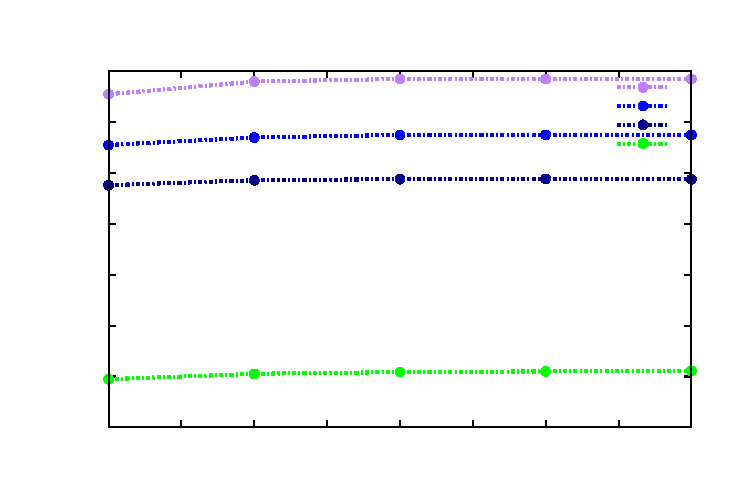
\includegraphics{./../graph/graphA}}%
    \gplfronttext
  \end{picture}%
\endgroup

        \caption{$V_{max}$ em função da intensidade}
        \label{graph:A}
    \end{subfigure}
 
    \begin{subfigure}{\linewidth}
        % GNUPLOT: LaTeX picture with Postscript
\begingroup
  \fontfamily{phv}%
  \selectfont
\definecolor{t}{rgb}{0.5,0.5,0.5}
  \makeatletter
  \providecommand\color[2][]{%
    \GenericError{(gnuplot) \space\space\space\@spaces}{%
      Package color not loaded in conjunction with
      terminal option `colourtext'%
    }{See the gnuplot documentation for explanation.%
    }{Either use 'blacktext' in gnuplot or load the package
      color.sty in LaTeX.}%
    \renewcommand\color[2][]{}%
  }%
  \providecommand\includegraphics[2][]{%
    \GenericError{(gnuplot) \space\space\space\@spaces}{%
      Package graphicx or graphics not loaded%
    }{See the gnuplot documentation for explanation.%
    }{The gnuplot epslatex terminal needs graphicx.sty or graphics.sty.}%
    \renewcommand\includegraphics[2][]{}%
  }%
  \providecommand\rotatebox[2]{#2}%
  \@ifundefined{ifGPcolor}{%
    \newif\ifGPcolor
    \GPcolortrue
  }{}%
  \@ifundefined{ifGPblacktext}{%
    \newif\ifGPblacktext
    \GPblacktextfalse
  }{}%
  % define a \g@addto@macro without @ in the name:
  \let\gplgaddtomacro\g@addto@macro
  % define empty templates for all commands taking text:
  \gdef\gplbacktext{}%
  \gdef\gplfronttext{}%
  \makeatother
  \ifGPblacktext
    % no textcolor at all
    \def\colorrgb#1{}%
    \def\colorgray#1{}%
  \else
    % gray or color?
    \ifGPcolor
      \def\colorrgb#1{\color[rgb]{#1}}%
      \def\colorgray#1{\color[gray]{#1}}%
      \expandafter\def\csname LTw\endcsname{\color{white}}%
      \expandafter\def\csname LTb\endcsname{\color{black}}%
      \expandafter\def\csname LTa\endcsname{\color{black}}%
      \expandafter\def\csname LT0\endcsname{\color[rgb]{1,0,0}}%
      \expandafter\def\csname LT1\endcsname{\color[rgb]{0,1,0}}%
      \expandafter\def\csname LT2\endcsname{\color[rgb]{0,0,1}}%
      \expandafter\def\csname LT3\endcsname{\color[rgb]{1,0,1}}%
      \expandafter\def\csname LT4\endcsname{\color[rgb]{0,1,1}}%
      \expandafter\def\csname LT5\endcsname{\color[rgb]{1,1,0}}%
      \expandafter\def\csname LT6\endcsname{\color[rgb]{0,0,0}}%
      \expandafter\def\csname LT7\endcsname{\color[rgb]{1,0.3,0}}%
      \expandafter\def\csname LT8\endcsname{\color[rgb]{0.5,0.5,0.5}}%
    \else
      % gray
      \def\colorrgb#1{\color{black}}%
      \def\colorgray#1{\color[gray]{#1}}%
      \expandafter\def\csname LTw\endcsname{\color{white}}%
      \expandafter\def\csname LTb\endcsname{\color{black}}%
      \expandafter\def\csname LTa\endcsname{\color{black}}%
      \expandafter\def\csname LT0\endcsname{\color{black}}%
      \expandafter\def\csname LT1\endcsname{\color{black}}%
      \expandafter\def\csname LT2\endcsname{\color{black}}%
      \expandafter\def\csname LT3\endcsname{\color{black}}%
      \expandafter\def\csname LT4\endcsname{\color{black}}%
      \expandafter\def\csname LT5\endcsname{\color{black}}%
      \expandafter\def\csname LT6\endcsname{\color{black}}%
      \expandafter\def\csname LT7\endcsname{\color{black}}%
      \expandafter\def\csname LT8\endcsname{\color{black}}%
    \fi
  \fi
  \setlength{\unitlength}{0.0500bp}%
  \begin{picture}(6802.00,4534.00)%
    \gplgaddtomacro\gplbacktext{%
      \csname LTb\endcsname%
      \put(774,576){\makebox(0,0)[r]{\strut{} 0.8}}%
      \put(774,1064){\makebox(0,0)[r]{\strut{} 1}}%
      \put(774,1552){\makebox(0,0)[r]{\strut{} 1.2}}%
      \put(774,2040){\makebox(0,0)[r]{\strut{} 1.4}}%
      \put(774,2529){\makebox(0,0)[r]{\strut{} 1.6}}%
      \put(774,3017){\makebox(0,0)[r]{\strut{} 1.8}}%
      \put(774,3505){\makebox(0,0)[r]{\strut{} 2}}%
      \put(774,3993){\makebox(0,0)[r]{\strut{} 2.2}}%
      \put(882,396){\makebox(0,0){\strut{} 5e+14}}%
      \put(1681,396){\makebox(0,0){\strut{} 5.5e+14}}%
      \put(2481,396){\makebox(0,0){\strut{} 6e+14}}%
      \put(3280,396){\makebox(0,0){\strut{} 6.5e+14}}%
      \put(4079,396){\makebox(0,0){\strut{} 7e+14}}%
      \put(4878,396){\makebox(0,0){\strut{} 7.5e+14}}%
      \put(5678,396){\makebox(0,0){\strut{} 8e+14}}%
      \put(6477,396){\makebox(0,0){\strut{} 8.5e+14}}%
      \put(144,2284){\makebox(0,0){\strut{}$V_{máx}$}}%
      \put(3679,126){\makebox(0,0){\strut{}frequência(Hz)}}%
      \put(3679,4263){\makebox(0,0){\strut{}$V_{max}$ em função da frequência incidente}}%
    }%
    \gplgaddtomacro\gplfronttext{%
      \csname LTb\endcsname%
      \put(2070,3840){\makebox(0,0)[r]{\strut{}dados}}%
      \csname LTb\endcsname%
      \put(2070,3660){\makebox(0,0)[r]{\strut{}regressão}}%
    }%
    \gplbacktext
    \put(0,0){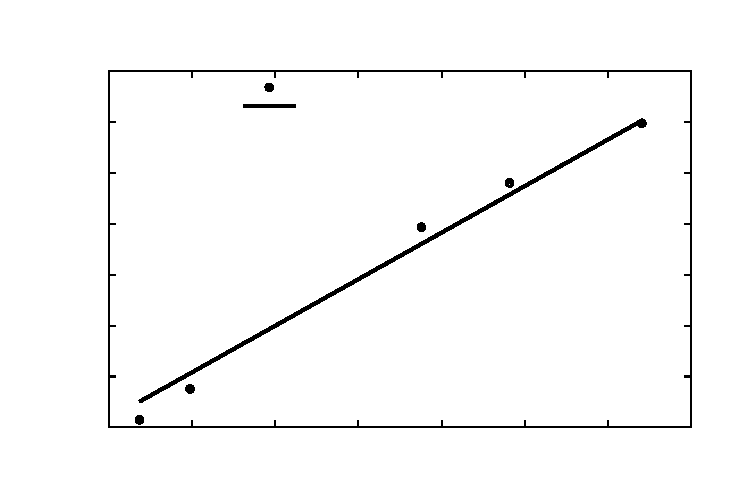
\includegraphics{./../graph/graphB}}%
    \gplfronttext
  \end{picture}%
\endgroup

        \caption{$V_{max}$ em função da frequência}
        \label{graph:B}
   \end{subfigure}
   \caption{ Gráficos}
\end{figure}
\FloatBarrier

\section{Conclusão}

\paragraph{}O experimento permitiu verificar algumas previsões da
física quântica ao mostrar que a energia cinética dos
fotoelétrons emitidos no efeito fotoelétrico é proporcional
a frequência incidente mas constante em relação a
intensidade. Foi possível medir a constante de Planck em $h
= (5.9\pm 0.5) \cdot 10^{-34}V$. Essa medida foi precisa,
pois o erro é de 6.8\%, mas não bateu com o valor tabelado e
portanto 
não foi acurada. Mediu-se também a função trabalho para o catodo 
utilizado em $W_0 = (1.6\pm 0.3) \cdot 10^{-19}V \cdot C$.
Essa medida não foi precisa por fornecer uma margem de erro
de 18.75\%.

%@@@@@@@@@@@@@@@@@@@@@@@@@@@@@@@@@@@@@@@@@@@@@@@@@@@@@@@@@@@
%@@@@@@@@@@@@@@       REFERÊNCIAS     @@@@@@@@@@@@@@@@@@@@@@
%@@@@@@@@@@@@@@@@@@@@@@@@@@@@@@@@@@@@@@@@@@@@@@@@@@@@@@@@@@@
\begin{thebibliography}{9}    
	 \bibitem{fis4-serway}
  		JEWETT, J.W.; SERWAY, R.A.
  		\emph{Física para cientistas e engenheiros}
volume 4 : Luz, Óptica e Física Moderna.
 		 8ª ed.
 		 São Paulo : Cengage Learning, 2012.
 		\end{thebibliography}
\end{document}
